
% This template can serve as a starting point for your MSc thesis. You are allowed to modify it as long as you adhere to the requirements from the Thesis Manual.
\documentclass[a4paper,11pt]{article}

% FILL OUT THE DETAILS BELOW:
\author{Minh Quang Ngo}
\title{T Enhancing Asset Pricing Models with Liquidity Factors and Sentiment: A Rule-Based Approach}
% \date{An optional custom date, the default is today}
\newcommand{\studentnumber}{597115}
\newcommand{\program}{Data Science and Marketing Analytics}
\newcommand{\supervisor}{Hakan Akyuz}
\newcommand{\secondassesor}{Name of your second assessor}

\usepackage[british]{babel} % Use British English
\usepackage[onehalfspacing]{setspace} % Increase line spacing
\usepackage[margin=2.5cm]{geometry} % Modify margins
\usepackage{graphicx,booktabs,apacite} % Packages for images, tables, and APA citations

% ADD YOUR OWN PACKAGES HERE
% Hint: \usepackage{amsmath,amsfonts,hyperref} imports some frequently used packages
\usepackage[utf8]{inputenc}
\usepackage{amsmath}

%drawing trees
\usepackage{tikz}
\usetikzlibrary{trees}

%cleverref
\usepackage{cleveref} 

%pdflandscae
\usepackage{pdflscape}


%%%%%%%%%%%%%%%%%%%%%%%%%%%%%%%%%%%%%
%%%%%%%%%%%END PREAMBLE################
%%%%%%%%%%%%%%%%%%%%%%%%%%%%%%%%%%%%%

\begin{document}

\begin{titlepage}
\makeatletter
\begin{center}
	\textsc{Erasmus University Rotterdam}
	\par \textsc{Erasmus School of Economics}
	\par Master Thesis \program

	\vfill \hrule height .08em \bigskip
	\par\huge\@title\bigskip
	\par\Large\@author\,(\studentnumber)\bigskip
	\hrule height .08em\normalsize
	
	\vfill
	
\includegraphics[width=\textwidth,height=0.15\textheight,keepaspectratio]{eur} % The EUR logo, but this could also be another image
	\vfill
	
	\begin{tabular}{ll}
		\toprule
		Supervisor: & \supervisor\\
		Second assessor: & \secondassesor\\
		Date final version: & \@date\\
		\bottomrule
	\end{tabular}
	
	\vfill
	The content of this thesis is the sole responsibility of the author and does not reflect the view of the supervisor, second assessor, Erasmus School of Economics or Erasmus University.
\end{center}
\makeatother
\end{titlepage}

%%%%%%%%%%%%%%%%%%%%%%%%%%%%%%%%%
%%%%%%%%CONTENT STARTS HERE%%%%%%%
%%%%%%%%%%%%%%%%%%%%%%%%%%%%%%%%%%%%%%%%%
\section{Introduction}
    
Asset-pricing models form the analytical backbone of modern finance: they turn noisy market data into estimates of expected returns and, by doing so, provide the foundation for portfolio construction, risk management, and capital-allocation decisions.  From the Capital Asset Pricing Model (CAPM) of \citeA{sharpe_1964} to the Fama-French Five-Factor (FF5) specification of \citeA{ff5_2015}, the standard practice has been to express expected returns as linear combinations of a small set of “risk factors.”  Despite their simplicity and enduring popularity, these linear models has been empirically shown to leave portions of the cross-section of returns unexplained and offer limited guidance when new sources of risk emerge.  Persistent mispricing anomalies and return premia that fall outside the span of the Fama French factors testify to these gaps and motivate the search for more robust modelling frameworks.

% Two economically intuitive dimensions of risk receive recurrent attention in the empirical literature yet remain under-represented in mainstream factor models. Liquidity risk captures the price impact and transaction cost penalties associated with trading in thin or stressed markets \cite{pastor_2003,acharya_2005}. Investor sentiment reflects systematic waves of optimism and pessimism that can temporarily decouple prices from the intrinsic value of companies \cite{wurgler_2007}.  A growing body of evidence shows that both dimensions command return premia and help explain well-known anomalies, suggesting that omitting them leaves valuable information on the table for academics and practitioners alike. Recent advances in machine learning point to a practical route for closing these gaps without sacrificing interpretability. In particular, we adopt the pseudo-beta framework of \citeA{simonian_2019}, which converts the variable importance of a RF ensemble into loadings that are conceptually analogous to OLS betas, thereby preserving the economic intuition of factor models while accommodating the non-linearities of liquidity and sentiment effects.

% Building on \citeA{simonian_2019}, this thesis investigates whether augmenting classical factor models with a superior specification such as RF can translate superior in-sample fit into actionable out of sample performance. Although Random Forests excel at capturing the non linear interactions between the so called `factor zoo', the sheer volume of their raw ensemble predictions offers little practical guidance for day to day portfolio allocation.  Association Rule Learning (ARL) closes this implementation gap by distilling those forecasts into a handful of transparent if-then rules, yielding deterministic signals that portfolio managers can audit, back-test, and communicate with ease. Equity sectors provide a natural arena for putting such rules to work.  Firms within a sector share common cash-flow drivers, regulatory settings, and macroeconomic sensitivities, so sector-level return dispersion is often pronounced even when aggregate market moves are calm. Because most institutional mandates already permit tactical deviations from a strategic sector benchmark, a sector rotation strategy based on ARL filtered Random-Forest signals integrates smoothly with existing governance frameworks and remains scalable at institutional capacity. 

These inconsistencies of the market remind both academics and practitioners that even the most preferred multifactor frameworks still omit economically important factors. Two such omissions stand out. Liquidity risk penalises investors forced to transact in thin or stressed markets, earning a premium that traditional factors only imperfectly capture \cite{pastor_2003,acharya_2005}. Investor sentiment in the form of optimism and pessimism could push prices away from its intrinsic value, affecting subsequent returns of equities \cite{wurgler_2007}. Ignoring these dimensions not only hampers our scientific understanding of the cross-section, but it also leaves exploitable information on the table for real-world portfolio construction.

Yet simply tacking new variables onto an ever-expanding “factor zoo" is not an easy task. What is needed is a modelling framework that (i) accommodates the non-linear interactions that liquidity and sentiment naturally exhibit, and (ii) preserves the economic intuition that has made linear factor models so influential. Recent machine-learning advances suggest a viable path. Ensemble methods such as Random Forests (RF) can flexibly learn complex return drivers, while post-hoc interpretation techniques such the pseudo-beta of \citeA{simonian_2019} can translate their output back into the language of betas. If those insights can be distilled into a handful of transparent rules, they could generate a sector-rotation overlay that fits seamlessly within institutional mandates. Accordingly, this thesis asks:

\textit{Can a machine-learning-augmented factor model both deepen our understanding of cross-sectional stock returns and generate an interpretable sector-rotation strategy that outperforms a broad market benchmark?}

which is answered via two sub-questions:
\begin{enumerate}
   \item[(a)] To what extent does enhancing classical multifactor asset-pricing models with additional liquidity and investor-sentiment indicators, improve out-of-sample explanatory and predictive power while preserving interpretability of the non parametric models?\\
  \item[(b)] How can the signals produced by such enhanced models be distilled into clear decision rules that guide sector rotation that outperforms S\&P500 index?\\
\end{enumerate}

To answer these questions, we (i) extend the C4F and FF5 models with liquidity and sentiment measures and translate Random Forest variable importance scores into pseudo-beta loadings following the framework of \citeA{simonian_2019}, (ii) compare out-of-sample explanatory and predictive performance across classical linear models, non-parametric specifications, and alternative RF implementations, and (iii) apply Association Rule Learning (ARL) to distill stable, interpretable pseudo-beta signals into daily sector rotation rules. By bridging the flexible explanatory power of machine learning with the transparency demanded by investment professionals, this study contributes both to academic debates on factor completeness and to the practical design of rule based allocation strategies. 


From an academic perspective, the study advances the machine learning and asset pricing literature in three ways. First, it is commonly understood that non-parametric models, while delivering high predictive power, cannot provide the same beta coefficients that finance practitioners require. Prior approaches to reconciling machine-learning accuracy with financial interpretability often relied on ad-hoc surrogate models or novel methods such as SHAP, which lack clear economic meaning. However, in this study, the rule set distilled from the Random Forest is interpreted with pseudo-betas and if-then conditions that restore the interpretability demanded by financial practitioners and regulatory oversight, while also delivering higher out-of-sample predictions than traditional Fama-French. Second, it extends the Random Forest rule extraction framework of \citeA{simonian_2019} by embedding liquidity risk per \citeA{pastor_2003} and an enhanced investor sentiment measure from \citeA{ung_2023} alongside the traditional Fama-French factors. By following a nonlinear analysis of these macroeconomic variables, the thesis overcomes the limited scope of prior studies and captures richer interactions among risk drivers. Third, unlike prior studies that focus primarily on in sample fit and static factor portfolios, this thesis presents rigorous out of sample evidence that interpretable machine learning factors can drive economically significant sector rotation strategies, thereby removing data-mining concerns and increasing the credibility of the expanding “factor zoo”. Collectively, these contributions bridge the academic gap between high accuracy yet opaque machine-learning approaches and tradidional asset pricing models. They demonstrate a practical path for incorporating rich macroeconomic variables into risk return frameworks without sacrificing transparency or theoretical coherence, and establishes the validity of actionable sector rotation strategies.


From a managerial perspective the decision rules extracted from RF forecasts are easily interpreted with a set of if-then conditions. They could then be integrated into dashboards and automated alerts to help portfolio managers and traders time sector rotation trades, scale positions ahead of liquidity squeezes and anticipate sentiment driven volatility spikes. This could also enable risk officers to adjust intraday execution algorithms and stress test funding liquidity scenarios, guiding corporate treasurers and investor relations teams in scheduling equity or debt issuance windows. The insights generated could also provide a real time marketing clock that enables analytics teams to synchronize strategic outreach with the market's risk and sentiment appetite. When the model projects a profitable next day excess return, campaign managers at financial institutions can push launches of the institutions'offerings such as high beta exchange traded funds, premium margin lending tiers, or thematic equity portfolios based on different sectors. For more traditional marketing analyst at these institutions, they could use the findings to schedule press releases and digital ads to coincide with heightened investor optimism. An example of this strategy in action is AllianceBernstein's launch of its clean energy thematic portfolio. According to AllianceBernstein's disclosures, the institution timed the public release to coincide with a period in which their own (more complex) model registered elevated the right market signals for the clean energy sector \cite{alliance_2024}. In practice the marketing analytics team initiated preparatory measures several months in advance by segmenting target client cohorts, designing phased email campaigns and reallocating digital-advertising budgets toward sustainability-focused creatives. As the model's excess-return forecast for clean energy crossed a certain threshold, the team accelerated client acquisition efforts and issued coordinated press releases, thereby ensuring that the market had already been primed when the real-time model signalled optimal conditions. Conversely, negative forecasted signal could prompt the platform to pivot messaging toward capital-preservation products, loyalty-focused retention workflows. The execution of this campaign is a prime example of how a rules-based framework like the one presented in this paper could be used to maximize the impact of marketing launch by aligning each tactical element with the evolving market risk and sentiment appetite. By converting advanced data science techniques into an interpretable rules based framework this thesis delivers an actionable tool that scales from the trading floor to the C suite.

The remainder of the study is organised as follows.  Section~\ref{sec:litrev} surveys the current literature on multifactor asset pricing models, machine-learning applications in finance, and the roles of liquidity risk and investor sentiment.  Section~\ref{sec:method} details the methodological framework, describing factor construction, the RF forecasting setup, and the ARL procedure that converts model outputs into sector rotation signals.  Section~\ref{sec:data} documents the data sources, sample selection and feature-engineering steps. Section~\ref{sec:results} presents the empirical results: model-interpretability diagnostics, forecasting comparisons, Diebold-Mariano tests, and the performance of both unconstrained and constrained rotation strategies. Finally, Section~\ref{sec:conclusion} concludes by discussing the findings in light of the research questions, highlighting limitations, outlining managerial implications, and suggesting directions for future research.

\section{Literature review}
	This literature review will examine the theoretical evolution of standard asset pricing models, beginning with the single-factor Capital Asset Pricing Model (CAPM) and extending to the multi-factor Fama-French frameworks. It will highlight the limitations of traditional statistical approaches in asset pricing and explore how advancements in machine learning methodologies may address these shortcomings. Then, the existing literature of the proposed enhancements to the asset pricing models will be reviewed. Specifically, the focus will be on the justification for incorporating liquidity risk and investor sentiment as explanatory factors. The ways in which contemporary researchers integrate these factors into their models will also be discussed. Furthermore, the application of asset pricing models within a sector rotation strategy will be explored, including an assessment of how this approach has been implemented in recent studies.


\subsection{A review of CAPM and its development}

The one factor Capital Asset Pricing Model (CAPM) of \citeA{sharpe_1964} was the first rigorious asset pricing framework, which relates an asset expected return to its market beta. Market beta measures the asset's systematic risk, or its sensitivity to fluctuations in the overall market. An assumption that CAPM makes is that investors hold mean-variance-efficient portfolios, or portfolios that offers the highest expected return for a given level of risk or, conversely, the lowest risk for a given level of expected return. This leads to the prediction that the expected return of an asset is linearly related to its market beta, with higher beta assets commanding higher expected returns as compensation for their increased exposure to market risk. Despite its theoretical appeal and widespread application due to its simplicity, empirical tests have revealed significant deviations from the model's predictions. Studies have found that a one factor could not explain certain stock return patterns. For example, small market capitalization (small-cap) stocks and high book to market ("value") stocks - or stocks that are undervalued- typically perform better than CAPM predicts \cite{capm_2004}.

In response to CAPM's shortcomings, \citeA{ff3_1993} introduced a three-factor model(FF3 hereafter) adding Size and Value factors in addition to the market factor. The motivation was based on earlier empirical findings that showed firm size and book-to-market equity robustly predict average returns, even when beta does not. By constructing portfolios to mimic these risk factors, the FF3 model significantly improved explanatory power. Indeed, in tests on U.S. stocks, the FF3 alphas (or the intercept of the linear regression model) were near zero, indicating that market, size, and value together “do a good job explaining the cross-section of average stock returns”. Size and value removes systematic mispricing present in the CAPM model. However, the FF3 still left some factors unexplained. \citeA{titman_2004} showed that firms with higher capital investments tend to experience lower future returns, a pattern not captured by the Fama-French three factors. \citeA{novymarx_2013} also found that the profitability of a firm could explain its expected return, similar to book-to-market ratio. Furthermore, some argue that there should be a momentum factor included in the asset pricing model.

\citeA{cahart_1997} introduces an extension of the FF3 by adding a momentum factor. The inclusion of the momentum factor is motivated by empirical evidence, which observes that stocks that have performed well in the past tend to continue outperforming, while past losers continue to underperform. Studies have shown that the size and value factors could not capture this effect. The Carhart 4 factor model (C4F hereafter) became a standard extension when the four factors could describe most of the cross-sectional returns. However, \citeA{huij_2009} indicates that the Carhart model proxies fail to account for real-world constraints. As a result, the premiums associated with the HML and momentum (PR1YR) factors tend to be misestimated.

With new emerging problems, \citeA{ff5_2015} propose a five-factor model (FF5 hereafter), adding profitability and investment factor.  The model does not include a momentum factor, as \citeA{ff5_2015} argue that momentum returns are largely short-term and difficult to reconcile with their asset pricing framework, which focuses on long-term risk premia. This update was motivated by research showing that firms with higher profitability or more conservative investment tend to earn higher returns. Interestingly, Fama and French in their own study found that the HML factor became less important in the presence of the new factors.  However, the five-factor model also had its limitations. It did not explicitly include momentum (so momentum remained an “external” anomaly), and it struggled with certain corner cases for instance, it failed to explain the low returns on small stocks that invest a lot despite low profitability. Both \citeA{sarwarff5} and \citeA{benammar_2018} concluded that the FF5 model cannot explain the average returns of US stocks. \citeA{cakici_2015} argued that the two additional factors are almost non-existent in large firms. With that said, there are tons of evidence of FF5's validity and robust explanatory power, in both national and regional studies \cite{sohor_litreview_2024}.

In sum, over decades the asset pricing model development (CAPM $\rightarrow$ FF3 $\rightarrow$ C4F $\rightarrow$ FF5) was driven by the need to address empirical gaps. Each new factor was added to account for a systematic return pattern unexplained by prior models. While these multifactor models capture much of the cross-section, research continues to find gaps, suggesting even more factors may be needed.


\subsection{Role of machine learning in factor models}

Despite the discourse between which model perfoms the best, one common characteristic they all have is that they are all linear models, which could potentially struggle with complex interactions or non-linear effects among predictors. \citeA{mcdonald_1962} highlights that traditional factor analysis methods assume linear relationships between manifest variables and latent factors, yet real-world financial markets often exhibit nonlinear interactions that linear models fail to capture. The author solidify this claim with another paper in 1983, which argue that factor models with polynomial regression functions, including interaction terms, provide a better framework that can accommodate these relationships \cite{mcdonald_1983}. As the research in ML produce better methods, the wave of its application in asset pricing started to come in. \citeA{hutchinson_1994}  provide one of the earliest applications of machine learning in finance by demonstrating how learning networks can be used for derivative pricing.More recent studies attempted to improve factor models return prediction performance. These ML methods can ingest a wide range of firm characteristics (including standard factors and many others) and capture nonlinear patterns. \citeA{gu_2020} provide a seminal example, applying various ML algorithms to predict the cross-section of U.S. stock returns. They find that flexible models, notably tree-based ensembles and neural networks substantially outperform linear methods in forecasting returns. \citeA{freyberger_2018} similarly show that a non-parametric ML approach uses far fewer predictors than a linear model yet attains a much higher out-of-sample Sharpe ratio indicating less overfitting and better true predictive power. \citeA{huynh_2023} used an LSTM-RNN algorithm to improve upon the FF5 predictive performance, solidifying the idea that ML models could empirically improve efficacy in portfolio management.

However, an improved predictive performance within ML models often comes with a decrease in interpretability,  leading to what is commonly known as the "black box" problem.Black-box models refer to algorithms whose internal decision-making processes are opaque or difficult for humans to understand. This is problematic in sectors where regulatory requirements and risk management demand transparency and accountability in decision-making \cite{brozek_2024}.  Moreover, financial markets are dynamic, and models trained on historical data may fail when market conditions change, a phenomenon known as "model drift". Therefore, it is essential to diagnose errors, biases or overfitting to historical data, which these black-box models cannot inherently do \cite{cohen_2021}. \citeA{lipton_2018} even critiques the common perception of linear models being inherently interpretable while deep neural networks are not. The author argues that interpretability depends on context, model complexity, and the availability of meaningful explanations. Several methods have been developed to mitigate the black-box problem by enhancing interpretability without significantly compromising predictive power. Model-specific approaches include decision trees and rule-based models, which allow users to enjoy the predictive power of black-box models while offering human-readable explanations. Feature importance techniques, such as SHAP (SHapley Additive exPlanations) and LIME (Local Interpretable Model-agnostic Explanations), analyze how individual input features contribute to model predictions. Other methods attempts to extract rules from the black box, such as surrogate trees which trains a more interpretable tree from the predictions of an ensemble. 



Building upon this body of research, \citeA{simonian_2019} introduced a ML approach to factor modeling by using the Random Forest (RF) algorithm on the C4F model. The authors argue that traditional factor models, including those used in commercial risk platforms, suffer from redundancy created by nonlinearity and multicollinearity. \citeA{simonian_2019} chose the RF model due to how RF could get rid of multicollinearity concerns while allowing for complex interactions. Furthermore, with the RF implementation, the author departs from the classical portfolio-sorting methodology, where stocks are first classified into groups (e.g., small-cap vs. large-cap) before factor loadings are estimated. Instead of forming factor-mimicking portfolios, RF treats each observation individually and evaluates how different factors contribute to returns at various points in time. To address the interpretability challenges inherent in ML-based factor models, \citeA{simonian_2019} incorporated feature importance metrics as an interpretable structure akin to $\beta$ coefficients in traditional factor model regressions. Additionally, they propose a method to construct pseudo-betas by weighting the raw factor elasticities with their respective relative feature importance (RFI hereafter) scores, effectively translating the RF model's output into a form that is more familiar to practitioners in finance. Beyond risk factor analysis, the interpretability of RF-derived predictions is used in a sector rotation strategy. Trading rules are established using RF predicted sector future return alongside volatility ratio signal. If both the predicted return exceeds a threshold and the short-term volatility is lower than long-term volatility, the sector is included in the portfolio. This research demonstrated how black-box models can be structured to provide actionable investment decisions while maintaining interpretability.

\subsection{Emerging additions to factor models}
An attractive feature of ML-enhanced models is their ability to incorporate a wide array of features that traditional econometrics models cannot - at least without constricting assumptions. This allows for the opportunity to include more factors within the factor models. Two factors that are frequently highlighted in the literature as valuable additions to factor models are liquidity risk and investor sentiment. The following discussion examines why these two factors are considered for asset pricing models and the findings when they are incorporated.

%%Maybe problems with factor zoo? 

\subsubsection{Liquidity Risk}
%%%%%Why liquidity is considered for asset pricing
A liquid investment can be bought and sold quickly without a significant change in its price. Liquidity risk occurs when the same investment faces an imbalance of buyers and sellers in the market or when external factors cause price volatility. \citeA{pastor_2003} provide strong empirical evidence that marketwide liquidity is a state variable that influences expected stock returns. Their study finds that stocks with higher sensitivities to liquidity fluctuations comes with a premium, as investors require additional compensation for holding assets that become difficult to trade when there is a decrease in liquidity. When liquidity "dries up" in the market, liquidity risk amplifies transaction costs and price impacts. Then, investors that use leverage or have liquidity constraints are almost "forced" into liquidating with a premium, further reinforce the pricing of liquidity risk. The authors also conducted a study on portfolios sorted on liquidity betas and found that there is still a significant spread on return, even after controlling for factors within the C4F model. \citeA{amihud_1986} argue that liquidity matters in asset pricing due to the bid-ask spread, which can represent the transaction cost that an investor can incur. Longer-term investors are more willing to hold less liquid assets because they amortize transaction costs over an extended period. Investors with shorter holding periods incur these trading costs more frequently, leading them to demand higher expected returns as compensation for illiquidity. The mechanism is simple: the more friction there is in trading securities, the more investors will want for holding them.\citeA{amihud_1986} confirm that assets with higher bid-ask spreads yield higher return, which adds evidence to liquidity being priced in the market. \citeA{amihud_2002} reinforced the findings, showing that when marketwide illiquidity is anticipated to rise, investors require higher forecasted stock returns. This occurs because higher expected illiquidity implies higher transaction costs and greater uncertainty, leading investors to discount prices accordingly. Additionally, higher status quo illiquidity raises expectations of future illiquidity, thereby increasing required returns and driving prices down. There has also been empirical evidence in international markets that CAPM and FF3 fail to explain stock returns in markets with significant liquidity premium such as Korea \cite{jang_2012}.Given this evidence, liquidity is not only a significant determinant of stock returns but also a systematic risk factor that should be incorporated into asset pricing models to improve their explanatory power.


%%% How are liquidity being implemented in asset pricing
\citeA{acharya_2005} extended the traditional CAPM by incorporating liquidity risk, stating that market risk must be accompanied by three additional risk factors: commonality in liquidity with the market, sensitivity of asset returns to market-wide liquidity fluctuations, and the tendency for an asset's liquidity to decline when the market is in distress. The authors find that the liquidity adjusted CAPM explains asset returns better than the standard CAPM, though not being able to fully explain the book-to-market effect. Findings by \citeA{amihud_1986,amihud_2002,pastor_2003} are also further reinforced. While \citeA{acharya_2005} introduced a liquidity-adjusted CAPM,\citeA{brennan_1998} explore how liquidity directly impacts returns through trading volume as a proxy of liquidity. The authors employ Fama-MacBeth regressions on individual securities rather than portfolios, isolating liquidity effects while adjusting for \citeA{ff3_1993} factors. The results further confirms that liquidity risk is priced in the market. The study finds that including trading volume in the asset pricing model reduces the SMB effect, as smaller firms are typically more illiquid. \citeA{li_2019} further investigates the findings of \citeA{pastor_2003}, successfully replicating their liquidity factor based on historical betas, but found that it is only marginally significant when controlling for other factors. The authors constructed tradable liquidity risk factors based on historical liquidity betas and predicted liquidity risk. When added to FF3, FF5 and CF4, predicted liquidity factor is not significant in any models, while historical liquidity betas is significant for FF3 and C4F. However, \citeA{li_2019} still concluded that asset pricing models are not substantially improved by adding a liquidity risk factor. \citeA{jang_2012} constructed a two-factor model specifically to explain the liquidity premium within the Korean stock market, which cannot be explained with CAPM or FF3. The proposed two factor model include market risk beta (as in CAPM) and a liquidity factor based on liquidity mimicking portfolio. In this specific market, the CAPM anomaly of small-cap stocks perfoming better than large-cap disappear, implying that the size premium is partially driven by liquidity risk. Furthermore, the liquidity factor captures the variation in returns among high and low book-to-market stocks, meaning that it better explains the value effect. This liquidity risk adjusted CAPM model even captured the anomalies better during the Asian financial crisis than both the CAPM and FF3.

\subsubsection{Investors' sentiment}

%%%%%%%%WHY SENTIMENT IS CONSIDERED FOR ASSET PRICING%%%%%

Traditional asset pricing models assumes competition among rational investor leads to equilibrium, which creates a market where asset prices exactly reflect their discounted cash flow. Even if individual investors operate irrationally, these so called "noise behavior" should self correct on an aggregate level \cite{friedman_1953}. However, scholars in behavioral finance state that the market do not agree with this theory, stating that participants that do not follow technical or fundamental analysis could heavily affect prices. These participants trade based on what the literature calls "investor sentiment". While definitions of investor sentiment vary across the literature, a widely accepted definition is provided by \citeA{wurgler_2007}, who describe it as "a belief about future cash flows and investment risks that is not justified by the facts at hand.". This sentiment can range from positive, neutral or negative based on market factors and global events. The ground theory for the effect of sentiment on stock returns is established with \citeA{delong_2019}'s research, which predicts that investor sentiment creates deviation from fundamental value even in the absence of risk : noise traders bear the risk that they themselves create, creating higher short-term return for them. \citeA{smales_2017} reinforces this notion and provided evidence for causality. The authors used a volatility index as a sentiment proxy and concluded that changes in this index preceded significant change in stock prices.


%%%%%%%%% HOW IS IT BEING IMPLEMENTED IN ASSET PRICING %%%%
These anomalies spurred researchers to empirically apply investor sentiment into asset pricing models. \citeA{wurgler_2007} developed a novel approach and demonstrated that speculative and hard to arbitrage stocks - small, young, high-volatility, unprofitable, non-dividend-paying, or distressed stocks - experience declining future prices following periods of high investor sentiment, and conversely, rising prices after periods of low sentiment. Positive sentiment leads to these stocks being overvalued and increase their demands, driving up its price before this mispricing correct themselves. The authors describe this phenomenon as a "sentiment seesaw" illustrating that the initial overvaluation of speculative stocks corresponds to an equivalent undervaluation of safer stocks, and vice versa. 

Common asset pricing models were also employed to find out the effect of sentiment on stock returns, one of which was the FF3. \citeA{stambaugh_2015} suggest that investor sentiment strengthen the negative relationship between idiosyncratic volatility and expected returns among overpriced stocks. The opposite could be observed for underpriced stocks. When the FF3 model is augmented with sentiment-based idiosyncratic volatility effects, the explanatory power for stock returns improves significantly. The findings suggest that the FF3 model underestimates the importance of sentiment and mispricing. \citeA{chung_2012} suggest that high investor sentiment during expansion periods leads to overpricing, particularly in small, volatile, and hard-to-value stocks, aligning with behavioral theories. The findings reinforce the role of investors' sentiment within asset pricing models. \citeA{tetlock_2017} constructed a pessimism factor and demonstrated that high levels of this factor would lead to a downward pressure on price using the SMB factor (among other factors) from the FF3 model. 


The most common asset pricing model that sentiment is applied to is the C4F. \citeA{wurgler_2006} found that the inclusion of SMB in regression generally reduces the sentiment predictions: small stocks are more influenced by sentiment. This highlights that size alone did not fully explain the cross-sectional patterns observed. On the other hand, sentiment-driven mispricing was distinct from the established momentum anomaly. Furthermore, they also argue against the classical models (CAPM), which attribute cross sectional returns to varying risks captured. \citeA{antoniou_2016} used Fama-Macbeth regressions on a sentiment-augmented CAPM, which is basically a C4F model with the addition of idiosyncratic volatility and analyst disagreement. Traditional CAPM predicts that higher beta stock should earn higher expected returns. However, the findings of this paper finds that this prediction only holds true in pessimistic sentiment periods. CAPM predictions are no longer true under optimism: higher beta stocks underperform low beta stocks. This phenomenon can be attributed to `noise trading' where investor overconfidence causes an overvaluation of high-beta stocks, resulting in these securities becoming overpriced and subsequently generating lower future returns. \citeA{fongtoh_2014} looks at an anomaly called `MAX', in which stock with high daily maximum returns previous month (high `MAX') have lower return with stocks that have low daily retunr last month (low `MAX'). Previous literature have proved that a long high `MAX' value-weighted portfolio and a short low `MAX' value weighted portfolio yields negative return according to C4F. The authors believe that this sentiment may play a role in this anomaly. When sentiment is incorporated, the authors found that this anomaly is explained by investors gambling behavior in low performing high MAX stocks.



All of these papers have in common is that there are no consensus definition on what investor sentiment is. Consequently, different sentiment measures were constructed across papers, complicating efforts to clearly identify which specific sentiment indicators should be incorporated into factor models. Nevertheless, there is a broad consensus in the literature that investor sentiment significantly influences stock price movements. Therefore, sentiment factors are increasingly incorporated into traditional factor models to enhance their predictive performance.




\section{Data}
	%stocks traded in SP500 from 2002 to 2024
%- CRSP %dsf crsp_a_indexes.dsp500list_v2})
    %- Amihud ill :permno, ret, vol 

The period of this research will be from 1990 until 2018, due to data availability and quality. Data for the most recent years are not included due to the COVID-19 pandemic, in which liquidity, sentiment and the economy of the entire world was affected. The main datasets in this thesis will be gathered from Wharton Research Data Services (WRDS)\footnote{https://wrds-www.wharton.upenn.edu} via Python API queries with the \texttt{wrds}, which contains all of the data points relating to liquidity risk,FF5/C4F factors and excess returns. The \texttt{permno}, or stocks the stocks' permanent identifier is specifically queried from the \texttt{crsp\_a\_indexes.dsp500list\_v2}
file. All of the other data points relating to liquidity risk, Fama-French factors and excess returns are either queried or calculated using the data points from the \texttt{crps.dsf} database. The sector classification is specifically derived from the \texttt{comp.company} file. With the same \texttt{gvkey, permno} keys, the datasets queried could be joined.

The enhanced sentiment index from the \citeA{ung_2023} is available directly from the paper's journal homepage, under "Supplemental Material" \footnote{https://doi.org/10.1080/1351847X.2023.2247440.}.


%more about the sentiment reddit thing on Paulus Pietiläinen thesis
\section{Methodology}
    %%%OUTLINE:%%%%

- liquidity risk factors construction
- sentiment construction
- fama and carhart models/factors 
- random forest
- Rule based model
- sector rotation strategy: Association rule learning

This chapter outlines the methodological approach adopted to measure liquidity risk and investors' sentiment, along with their rationale. These factors are integrated into an enhanced asset pricing framework based on the FF5 and C4F. Subsequently, the implementation of the Random Forest (RF) algorithm is detailed. Next, the rule-based model will be extracted from the RF for comparison and application to the Association Rule Learning Sector Rotation Strategy.

\subsection{Liquidity Risk factor}
%%%%% ACTUAL%%%%%%%%%%%
The construction of liquidity factors closely align with the methodology outlined by \citeA{gu_2020}. The authors include multiple liquidity related variables, including turnover and turnover volatility (\texttt{turn}, \texttt{SDturn}), log market equity (\texttt{mvel1}), dollar volume (\texttt{dolvol}), Amihud illiquidity (\texttt{ILLQ}), number of zero trading days (\texttt{zerotrade}), and bid-ask spread (\texttt{baspread}). \citeA{amihud_2002} defined their illiquidity measure \texttt{ILLQ} as the "average ratio of the daily absolute return to the(dollar)trading volume on that day. This index captures waves of excessive optimism or pessimism in the market.  The calculation for Amihud illiquidity is as follows:

\begin{equation}
    \label{eq:amihud}
    \text{ILLIQ}_{i,y} = \frac{1}{D_i^y} \sum_{d=1}^{D_i^y} \frac{|R_{i,d}|}{VOL_{i,d}}
\end{equation}
    
with $R_{i,d}$ being the return on stock $i$ on day $d$. $VOL_{i,d}$ being trading volume (in dollars) for stock $i$ on day $d$ and $D_i^{y}$ being the number of days for which data is available for stock $i$ in year $y$. \citeA{amihud_2002} suggested that this measure be multipled with the ratio of $10^6$, as the ratio would be tiny. Each stock-level liquidity characteristic is cross-sectionally ranked period-by-period, then mapped into a standardized interval ranging from -1 to 1 \cite{gu_2020}. 

%(is batch normalization needed?)

%Add a part that says unlike the literature on this topic, no portfolio sorting is needed.

\subsection{Sentiment}
%% OUTLINE: wurgler -> antoniu -> XU enhanced
\citeA{wurgler_2006} constructed a sentiment index (BW index hereafter) by capturing the principal components within six proxies: closed-end fund discount (\texttt{CEFD}), NYSE share turnover (\texttt{TURN}), the number and average first-day returns of IPOs (\texttt{NIPO, RIPO} respectively), equity share in new issues (\texttt{S}) and dividend premium (\texttt{P}). \footnote{However, by March 2016, the NYSE share turnover proxy has been dropped in the database due to "the explosion of institutional high-frequency trading and the migration of trading to a variety of venues" \cite{ung_2023}}%can definitely add more after the proposal here, from the paper

The sentiment is calculated as follows:
\begin{equation}
    \label{eq:sentiment}
    \begin{split}
    \text{SENTIMENT}_t = -0.241\,\text{CEFD}_t + 0.242\,\text{TURN}_{t-1} \\ + 0.253\,\text{NIPO}_t 
    + 0.257\,\text{RIPO}_{t-1} \\ + 0.112\,S_t - 0.283\,P^{D-ND}_{t-1} , 
    \end{split}
\end{equation}

where each proxy has been standardized. $\text{D}-\text{ND}$ is the difference between dividend payers and non-dividend payers. Principal Component Analysis(PCA) reveals the hidden common factor from this group of factors by transforming the data into principal components (PCs) that would capture as much variance in the data as possible. PC1 should capture the maximum variation from the sentiment proxies, thereby serving as an aggregate measure of investor sentiment. Since both market sentiment and the business cycle can drive common variation in financial data, the PCA will treat both as sources of variance without distinguishing whether that variance comes from changes in investor sentiment or broader macroeconomic factors. A second orthogonalized index is formed by regressing each of the proxy with independent variables that explains the business cycle. The residuals of this regression will be the "pure" sentiment, which is the variation that the macroeconomic factors fail to explain. The following is the orthogonalized index, with $\perp$ labelling the removal of business cycle. 

\begin{equation} %BEQ
    \label{eq:sentiment_orth}
    \begin{split}
    \text{SENTIMENT}^{\perp}_t = &-0.198\,\text{CEFD}^{\perp}_t + 0.225\,\text{TURN}^{\perp}_{t-1} \\
    &+ 0.234\,\text{NIPO}^{\perp}_t + 0.263\,\text{RIPO}^{\perp}_{t-1} \\
    &+ 0.211\,S^{\perp}_t - 0.243\,\text{P}^{\text{D} - \text{ND},\perp}_{t-1}
    \end{split}
\end{equation}

However, \citeA{ung_2023} pointed out several problems with the BW index. First, though it has robust predictive perfomance on a cross- sectional level, it is weak for aggregate market retuerns in time series regressions - even \citeA{wurgler_2007} pointed this out themselves in the paper. Second, the BW index assumes that the contributions of each sentiment proxy to the aggregate index are fixed over time. Finally, the index has `look ahead bias': PCA uses the whole sample, and forecasts at time $t$ should not rely on data that would only become available after $t$. Therefore, \citeA{ung_2023} constructed an enhanced index to address these problems. The time-varying BW sentiment index ($S^{TV}$ hereafter) is constructed on a three years rolling window basis to use the most up-to-date information at each $t$, and is built upon \cref{eq:sentiment_orth}. This rolling window allows the model to adjust to structural breaks in the market without distorting the sentiment index. Furthermore, adjustments to the sign of the RICO proxy display a negative initial loading. This paper will use \citeA{ung_2023} $S^{TV}$ index to measure investors' sentiment.


\subsection{Factor models}
%%%%%%%%OUTLINE%%%%%%%%%%
- Fama French 3
- Fama Carhart 4
- Fama French 5

- Factor models are generally linear. Which kinds of regression are they usally used with (fama macbeth)? 
- Since there are debate for which factor model is best, we want to test FF3, C4F and FF5

Time series regression on six asset pricing models.

Seven factor model:

\[
R_{it} - R_{Ft} = \alpha_i + \beta_1 \text{MktRF}_t + \beta_2 \text{SMB}_t + \beta_3 \text{HML}_t + \beta_4 \text{RMW}_t + \beta_5 \text{CMA}_t + \beta_6 \text{IML}_t + \beta_7 \text{LR}_t, \quad (6)
\]

I am going to run also the sentiment index on this too, so 8 factors

" Linear
models are preferred by practitioners because they gen-
erally present readily understandable and interpretable
analysis. In contrast, machine learning approaches,
although useful in uncovering the nonlinear behavior
of and interaction relationships among variables, are
often articulated in a way that makes their output unin-
tuitive, and hence unattractive, to many investment pro-
fessionals. "

Also, you don't even need to do the portfolio sortings like in thesis

Instead of just looking at the average effect of factors, analyzing different percentiles helps us understand how factors behave across low, median, and high return environments.

We are going to do this with the portfolios constructed before, so no need for percentiles


Random Forest Importance compares how important each feature is comparing to others in the same set, it is very useful to offer portfolio guidance such as in  return based style analyis (RBSA). he RF model, however,
possesses an advantage over a standard RBSA in gener-
ally providing a much better fit,

"Because the RF model captures hierarchical
(non-geometric) relationships between factors, it cannot
be understood as a direct analog of an OLS regression
or PCA because it does not convey the individual direc-
tional relationships between factors and assets."

We have to attempt to "beta-tize" the random forest. Beta is basically the elasticity of one variable to another. What we can do is to divide the predicted target variable return by each pre-
dictor return to gain a raw elasticity value for each factor.

\subsection{Liquidity proxy}

\textbf{Amihoud illiquidity ratio and Liquidity factor portfolio}
$$\text{Illiquidity} = \text{Average} \left( \frac{|R_{iyd}|}{\text{VOLUME}_{iyd}} \right)
$$

%%%%%%%%%%ACTUAL%%%%%%%%
One widely used metric is the Amihud illiquidity measure, which measures the price impact of trading. It could be intuitively understood as how much prices move per unit of volume - higher values mean the stock is harder to trade without moving the price. Amihud also found a significant illiquidity premium, which are stocks with higher Amihud's illiquidity values earn higher average returns, presumably compensating investors for bearing liquidity risk. In his cross-sectional tests, expected stock returns increased with expected illiquidity \cite{amihud_2002}


1.
- Use this for every single stock listed on the SP500 on a day as a proxy for stock illiquidity. Multiply this ratio by 10 to power 6. 
- Calc the moving average monthly (21 trading days). The first trading day of the month will thus capture the average illiquidity ratio of the previous month.

2.
- Fama and French approach: Sort the stock based on market cap into 2 groups: small and big (This is basically the SMB variable)
- Then the stock is INDEPENDENTLY sorted based on their illiquid ratio into 5 groups.Each stock is value weighted, meaning that stocks with a higher marketr capitalization gets a larger weight in the portfolio
- Now we have $2*5=10$ value weight portfolio based on size and illiquidity


3.
Now we need to construct long-short liquidity factor portfolio:

- Long illiquid portfolios
- Sell most liquid portfolios

A liquidity long-short portfolio is a trading strategy that profits from the difference in returns between illiquid and liquid stocks

This can be verified with the liquidity factor return, or just the excess return for holding illiquid stocks

$$
\text{Liquidity Factor Return} = \frac{1}{2} \left( R_{S5} + R_{B5} \right) - \frac{1}{2} \left( R_{S1} + R_{B1} \right)
$$
Where:

- \( R_{S5} \) and \( R_{B5} \) are the returns of the **most illiquid** small and big portfolios.
- \( R_{S1} \) and \( R_{B1} \) are the returns of the **most liquid** small and big portfolios.



This whole thing captures the return premium associated with illiquidity. Stocks that are harder to trade often earns higher returns


In addition to the 10 illiquidity portfolios, lets compute illiquidity portfolios based on size. I first sort the stocks on their firm's market capitalization in two groups, and afterward sort stocks on their illiquidity measure in their size group. This creates five illiquidity portfolios for small stocks and five illiquidity portfolios for big stocks.



\textbf{Fama French Five Factors models}

The following are its factors:

CAPM
- Market risk Factor from NYSE, NASDAQ and AMEX (Data taken from CRSP)

Before constructing the factors, Fama and French make 
1. six value weighted on size (small or big) and book to market ratio (value, neutral, growth)
2. six value weighted on size and operating profitability (robust, neutral, weak )
3.six value weighted on size and ivestment activity

Fama french 3
- Size factor (SMB)
    - The SMB factor is computed by subtracting the average return of the nine big stock portfolios
    (Big Value, Big Neutral, Big Growth, Big Robust, Big Neutral, Big Weak, Big Conservative,
    Big Neutral, and Big Aggressive) from the average return of the nine small stock portfolios
- Value factor (HML)
    -  spread between the average of the two value portfolios and the average of the two growth portfolios

Fama French 5
- Robust minus weak (RMW)
    - calculated by subtracting the average return of the two
    weak operating profitability portfolios from the average return of the two robust operating
    profitability portfolios.
- Conservative minus aggressive (CMA)
    - the difference between the average return of
    the two conservative investment portfolios and the average return of the two aggressive
    investment portfolios 

- Excess returns:
    - Return -risk free rate (RF from the kenneth data)

\subsection{Sentiment}
Enhanced investor sentiment dataset (Sze Nie Ung)








\textbf{Sector rotation strategy}

Apply RF variant to build a sector rotation strategy using ARL (Association rule learning). We can use this to deduct inference rule from epirical data

- RL is a rolling-window learning approach, meaning it continuously updates its understanding of market conditions.
Instead of using a fixed model trained once on historical data, it adapts dynamically by re-estimating relationships every 18 months.
This helps capture changing market dynamics—for example, a factor that worked last year may not work the same way today

Two signals are used:
- Random forest predicted excess within a portfolio
- Ratio of shorter-term to longer-term realized volatility (24-month vs. 36-month)

iterative add factor de xem la feature importance co doi ko 
\section{Planning}



\begin{landscape} % Begin landscape mode
	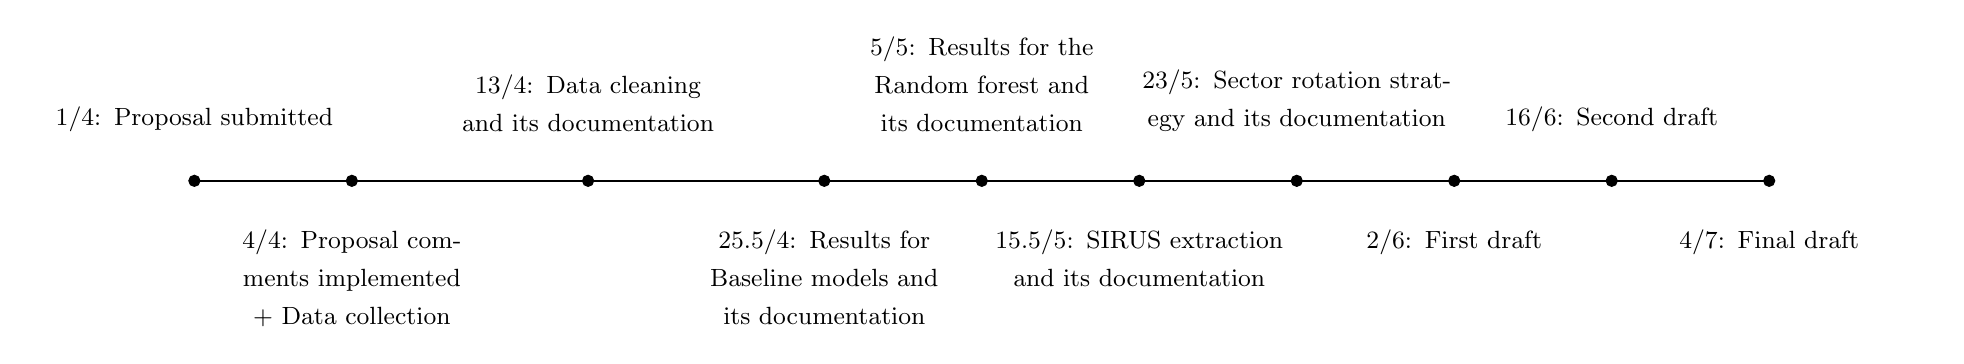
\begin{tikzpicture}[x=1cm, y=1cm, every node/.style={font=\small}]
	
		% Draw the horizontal timeline line
		\draw[thick] (0,0) -- (20,0);
		
		% Define styles for nodes above and below the timeline with fixed text width
		\tikzset{
			timeline above/.style={above=5mm, align=center, text width=4cm},
			timeline below/.style={below=5mm, align=center, text width=4cm}
		};
		
		% Event 1 (above): 1/4: Proposal submitted
		\draw[fill] (0,0) circle (2pt);
		\node[timeline above] at (0,0) {1/4: Proposal submitted};
		
		% Event 2 (below): 1/4-7/4 with midpoint 4/4: Proposal comments implemented + Data collection
		\draw[fill] (2,0) circle (2pt);
		\node[timeline below] at (2,0) {4/4: Proposal comments implemented + Data collection};
		
		% Event 3 (above): 8/4-19/4 with midpoint 13/4: Data cleaning and its documentation
		\draw[fill] (5,0) circle (2pt);
		\node[timeline above] at (5,0) {13/4: Data cleaning and its documentation};
		
		% Event 4 (below): 21/4-30/4 with midpoint approx.\,25.5/4: Results for Baseline models and its documentation
		\draw[fill] (8,0) circle (2pt);
		\node[timeline below] at (8,0) {25.5/4: Results for Baseline models and its documentation};
		
		% Event 5 (above): 1/5-9/5 with midpoint 5/5: Results for the Random forest and its documentation
		\draw[fill] (10,0) circle (2pt);
		\node[timeline above] at (10,0) {5/5: Results for the Random forest and its documentation};
		
		% Event 6 (below): 12/5-19/5 with midpoint 15.5/5: SIRUS extraction and its documentation
		\draw[fill] (12,0) circle (2pt);
		\node[timeline below] at (12,0) {15.5/5: SIRUS extraction and its documentation};
		
		% Event 7 (above): 20/5-26/5 with midpoint 23/5: Sector rotation strategy and its documentation
		\draw[fill] (14,0) circle (2pt);
		\node[timeline above] at (14,0) {23/5: Sector rotation strategy and its documentation};
		
		% Event 8 (below): 2/6: First draft
		\draw[fill] (16,0) circle (2pt);
		\node[timeline below] at (16,0) {2/6: First draft};
		
		% Event 9 (above): 16/6: Second draft
		\draw[fill] (18,0) circle (2pt);
		\node[timeline above] at (18,0) {16/6: Second draft};
		
		% Event 10 (below): 4/7: Final draft
		\draw[fill] (20,0) circle (2pt);
		\node[timeline below] at (20,0) {4/7: Final draft};
	\end{tikzpicture}
	
	In addition to the timeline provided, I intend to frequently send my current work to Professor Akyuz for feedback. Meaning, for each of the steps listed in the timeline, the latest update to the first draft of the thesis will be sent to Professor Akyuz. While waiting for his feedback on a particular section, I will continue to work on the next section.
\end{landscape}




\newpage
\bibliographystyle{apacite} 
\bibliography{ref_masterthesis.bib} 

\newpage
\appendix
\section{Appendix}
\subsection{Github repository}

\end{document}